\documentclass[herrin-thesis.tex]{subfiles}
\begin{document}
\section{History}
\subsection{Beta Decay}
Neutrino physics first arose in the study of beta decay. In the most basic form of beta decay, a neutron in the nucleus decays to a proton and emits an electron. \todo{Who first found a continuous spectrum for the electron?}Early nuclear physicists discovered that unlike alpha particles and gamma rays, which are emitted in monoenergetic lines from nuclear processes, beta decay electrons were emitted with a continuous range of energies. Rather than abandoning the principle of energy conservation, Wolfgang Pauli\addref in 1930 proposed a massless particle that could carry away the ``missing energy'' in beta decays. In 1933, Enrico Fermi\addref combined the idea with Heisenberg's nucleon model to form a theory of beta decay.

\subsection{Discovery}
For several decades after Pauli proposed the neutrino, the only evidence for its existence was indirect, through momentum and energy conservation. It was not until 1956 that Cowan and Reines\addref observed the electron antineutrino. Their experiment consisted of a large tank of water with cadmium chloride dissolved. Electron antineutrinos from a nearby nuclear reactor would interact with protons in the water molecules, creating a positron and a neutron. In the experiment, the positron annihilated, producing gamma rays. Cadmium is a good neutron absorbed, and the capture created another gamma ray. The delayed coincidence of the two gamma rays provided evidence of inverse beta decay.

The discovery of the muon in 1936 provided the possibility of a muon neutrino, distinct from the electron neutrino. In 1962, Lederman, Schwartz, and Steinberger\addref showed that a beam of neutrinos, created from a beam of decaying pions, aways interacted to form muons and not electrons. We now know that each charged lepton forms an isospin doublet with its associated neutrino.

\subsection{The Solar Neutrino Problem}

\subsection{Evidence for Oscillation}

\section{Theory of Massive Neutrinos}
\subsection{Constraints on Mass}

\subsection{Majorana Particles}

\subsection{Double Beta Decay}

\begin{figure}
	\centering
	\begin{subfigure}[b]{0.48\textwidth}
		\centering
		\includegraphics[width=\textwidth]{./feynman_diagrams/twonubetabeta.pdf}
		\caption[Diagram of \(2\nu\beta\beta\)]{The standard model allowed mode of two neutrino double beta decay.}
		\label{fig:diagram_2nubb}
	\end{subfigure}\hfill%
         \begin{subfigure}[b]{0.48\textwidth}
		\centering
		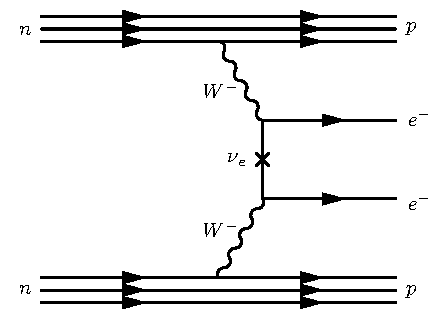
\includegraphics[width=\textwidth]{./feynman_diagrams/zeronubetabeta.pdf}
		\caption[Diagram of \(0\nu\beta\beta\)]{The neutrinoless mode of double beta decay.}
		\label{fig:diagram_0nubb}
	\end{subfigure}
	\label{fig:diagrams}
	\caption[Double beta decay modes]{Double beta decay modes}
\end{figure}

\end{document}